\documentclass[10pt,twocolumn,letterpaper]{article}

\usepackage{iccv}
\usepackage{times}
\usepackage{epsfig}
\usepackage{graphicx}
\usepackage{amsmath}
\usepackage{amssymb}

%%addied by shubham
\usepackage{caption}
\usepackage{booktabs}
\usepackage{multirow}
\usepackage{ctable}
\newcommand{\overbar}[1]{\mkern 1.5mu\overline{\mkern-1.5mu#1\mkern-1.5mu}\mkern 1.5mu}
\newcommand*\samethanks[1][\value{footnote}]{\footnotemark[#1]}
\usepackage{subcaption}
% \usepackage{subcaption}
%%end added by shubham %%

% Include other packages here, before hyperref.

% If you comment hyperref and then uncomment it, you should delete
% egpaper.aux before re-running latex.  (Or just hit 'q' on the first latex
% run, let it finish, and you should be clear).
\usepackage[pagebackref=true,breaklinks=true,letterpaper=true,colorlinks,bookmarks=false]{hyperref}

% \iccvfinalcopy % *** Uncomment this line for the final submission

\def\iccvPaperID{2171} % *** Enter the ICCV Paper ID here
\def\httilde{\mbox{\tt\raisebox{-.5ex}{\symbol{126}}}}

% Pages are numbered in submission mode, and unnumbered in camera-ready
\ificcvfinal\pagestyle{empty}\fi
\begin{document}

%%%%%%%%% TITLE
\title{High Accuracy Face geometry Capture using a Smartphone Video}

\author{First Author\\
Institution1\\
Institution1 address\\
{\tt\small firstauthor@i1.org}
% For a paper whose authors are all at the same institution,
% omit the following lines up until the closing ``}''.
% Additional authors and addresses can be added with ``\and'',
% just like the second author.
% To save space, use either the email address or home page, not both
\and
Second Author\\
Institution2\\
First line of institution2 address\\
{\tt\small secondauthor@i2.org}
}

% \maketitle
%\thispagestyle{empty}

\twocolumn[{%
\renewcommand\twocolumn[1][]{#1}%
\vspace{-1em}
\maketitle
\vspace{-1em}
\begin{center}
   \centering 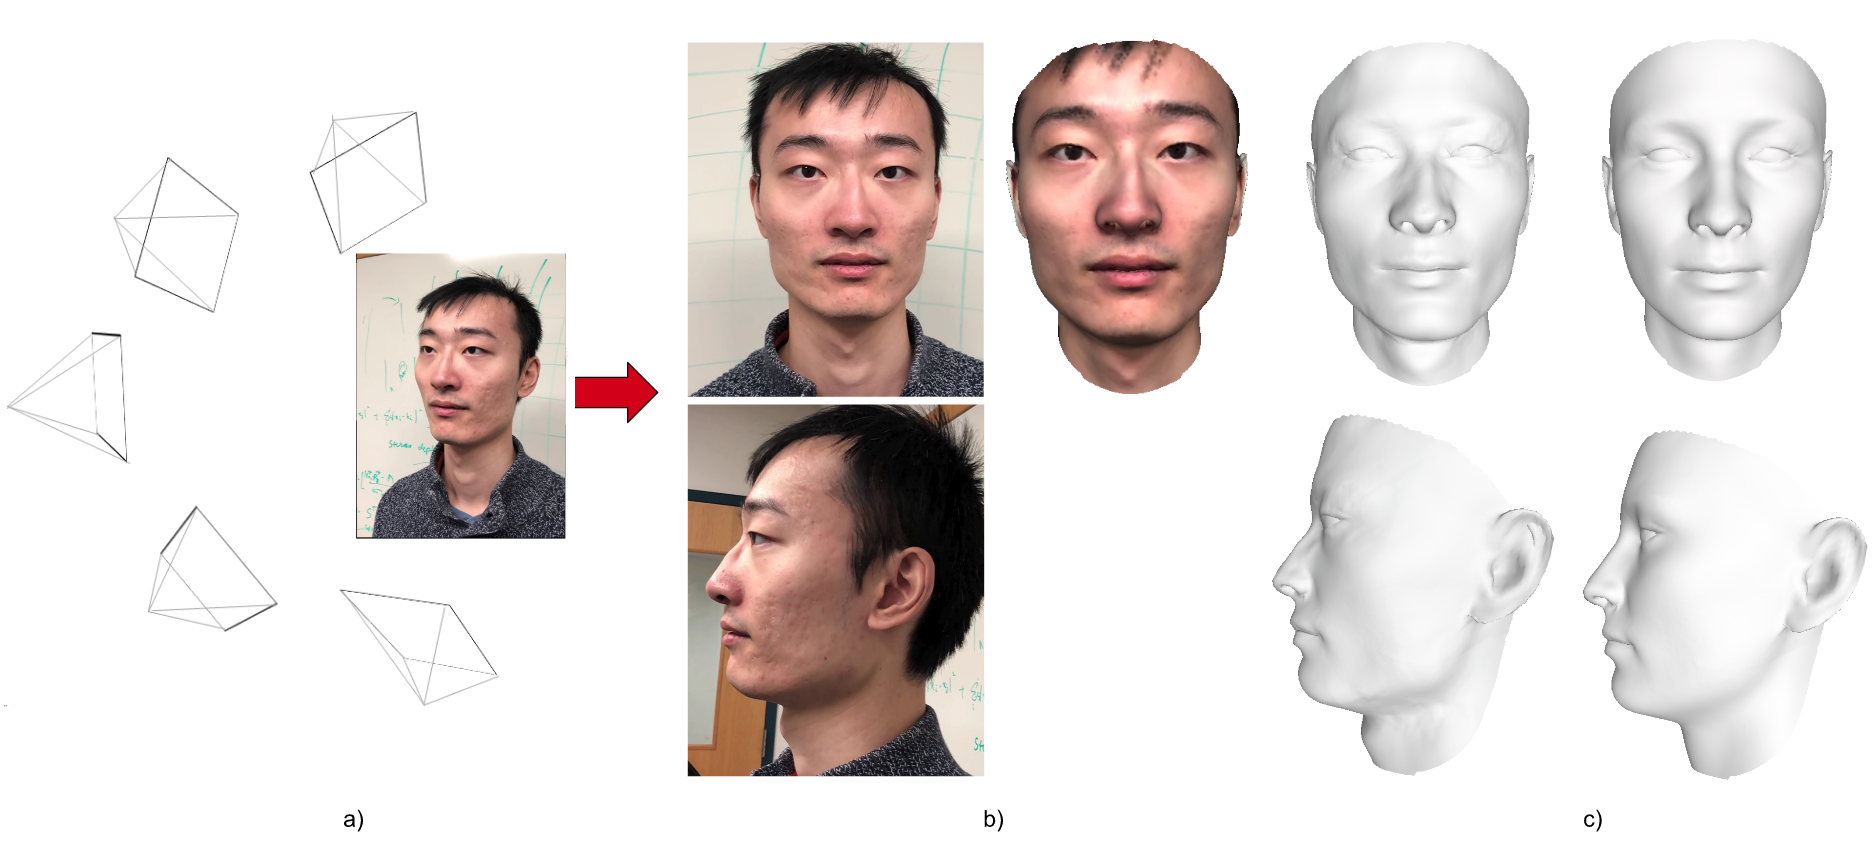
\includegraphics[width=\textwidth]{../images/cover_chaoyang.png} \captionof{figure}{a) Our method uses a single video clip of a subject taken in an unconstrained environment to reconstruct a high accuracy mesh of the face geometery. b) Our textured mesh side-by-side with input rgb image c) Our method (left) compared to the state-of-the-art method of \cite{hernandez2017accurate}(right), front and profile view.}
   \label{cover}
\end{center}%
}]


%%%%%%%%% ABSTRACT
\begin{abstract}
   The ABSTRACT is to be in fully-justified italicized text, at the top
   of the left-hand column, below the author and affiliation
   information. Use the word ``Abstract'' as the title, in 12-point
   Times, boldface type, centered relative to the column, initially
   capitalized. The abstract is to be in 10-point, single-spaced type.
   Leave two blank lines after the Abstract, then begin the main text.
   Look at previous ICCV abstracts to get a feel for style and length.
\end{abstract}

%%%%%%%%% BODY TEXT
\section{Introduction}


Reconstructing faces has been a problem of great interest in computer vision and graphics with applications in a wide variety of domains, ranging from animation \cite{ichim2015dynamic}, entertainment \cite{saito2016real}, genetics, biometrics, and more recently, augmented and virtual reality. Despite the long body of work, 3D face reconstruction still remains an open and challenging problem, primarily because the high level of detail required owing to our sensitivity to facial features. Even slight anomalies in the reconstructions can make the output look unrealistic and hence, accuracy of reconstructed face models is of utmost importance.


The seminal work of Beeler \etal \cite{beeler2010high} used a studio setup of cameras to capture face geometry accurately. Since then, a variety of work has focused on using Photometric stereo or Multi-view stereo techniques in studio settings for face reconstruction and performance capture \cite{cao2018sparse, fyffe2017multi}. 
Although accurate in their reconstructions, these studio setups are not trivial to setup, typically requiring a calibrated camera setup along with controlled lighting and backgrounds. This makes them infeasible for capturing `in-the-wild' subject faces in unconstrained settings, for instance an end user of a virtual reality app. For the purposes of animation or modeling, accurate 3D scans can be obtained from structured light or laser scanners, which are often prohibitively expensive, typically costing tens of thousands of dollars. 

To tackle the problem of unconstrained 3D face reconstruction, the community has mostly relied on three-dimensional morphable models (3DMMs)~\cite{blanz1999morphable}. 3DMMs are low-dimensional linear subspaces of faces typically constructed using a small set of ground truth 3D scans that enable rapid approximation of face geometry, typically through a combination of appearance based and landmark based optimization. In recent years, there has been a lot of interest in using deep neural nets to fit morphable models using a single image. However, single view depth estimation is a fundamentally ill-posed problem. Coupled with the reliance on synthetic data, generalization to in-the-wild images is often a concern for these methods. Often, while the results are visually appealing with texture, the reconstructions suffer from high geometric inaccuracies.

With the limited availability of 3D data for faces, using geometric cues from multiple views to improve accuracy of reconstruction becomes necessary. Previous work has shown that a single template or 3DMM can be optimized using constraints from multiple views, using techniques like photometric stereo \cite{roth2015unconstrained} or advances in automatic keypoint detection \cite{huber2016multiresolution}.
Recently, Hernandez et. al \cite{hernandez2017accurate} proposed an elegant multi-view constrained structure-from-motion scheme that explicitly optimized the coefficients of a 3DMM shape to recover face geometry. However, the output still remains constrained to the underlying training data and low capacity of the 3DMM. This greatly limits its expressivity, and is particularly undesirable for medical or biometric usage. 


In this work, we attempt to answer the question ``What's the most accurate reconstruction an end-user can obtain, without needing access to special equipment or studio setups?". To this end, we propose a pipeline for highly accurate yet robust face geometry capture, requiring nothing but a smartphone. We leverage recent advances in the fields of object and keypoint detection, direct methods for visual SLAM, and high-frame rate capture functionality available on modern smartphones to propose a pipeline that achieves state-of-the-art geometric accuracy among unconstrained face reconstruction techniques.

Our major contributions are as follows:
 \begin{itemize}
     \item  A principled reconstruction pipeline that takes a single video of a subject's face and reconstructs their face geometry with high fidelity. The reconstructed meshes are in dense semantic correspondence without beign constrained to any model subspace, making them ideal for usage in downstream tasks like animation, printing, genetic analyisis/modeling, biometrics etc. We make the code public, allowing anyone to be able to obtain accurate reconstructions of faces
     \item A collected dataset of 200 high-frame-rate  sequences of 100 individuals, where we collect two sequences per subject, under varying lighting conditions.
 \end{itemize}

\section{Prior Work}
Prior work on 3D Face Reconstruction is substantially large and a complete literature review is out of scope for the paper. Here, we talk about about some of the works closely related to ours.

\noindent \textbf{SfM based Multi-view Reconstruction.} A lot of multi-view reconstruction methods employ a Structure-from-Motion pipeline ~\cite{gotardo2015photogeometric, lin2010accurate, fidaleo2007model} but with unconvincing results on unconstrained in-the-wild videos ~\cite{hernandez2017accurate}. ~\cite{brand2001morphable} and ~\cite{shi2014automatic} use 3D Morphable Model~\cite{blanz1999morphable} for fitting shapes on every frame after computing correspondances among them. This restricts the reconstruction to a low-dimensional linear subspace. Hernandez ~\etal ~\cite{hernandez2017accurate} use 3DMM as a prior instead to search for correspondances among frames. This allowed them to achieve state-of-the-art results in unconstrained multi-view face reconstruction. However their method requires camera intrinsics to be known and the output is still constrained to a linear basis. We use this method as one of the baselines for comparison.

\noindent \textbf{Photometric Stereo.} Photometric stereo based methods have proven effective for large unconstrained collection of photos ~\cite{kemelmacher2011face, kemelmacher2013internet, roth2015unconstrained}. ~\cite{kemelmacher2011face} generates a 2.5D face surface by using SVD to find the low rank spherical harmonics. Roth \etal ~\cite{roth2015unconstrained} expand on it to handle pose variations and the scale ambiguity prevalent in the former method. They further expand their work in ~\cite{roth2016adaptive} where they fit a 3DMM to 2D landmarks for every image and optimize for the lighting parameters rather than SVD based factorization. Suwajanakorn ~\etal ~\cite{suwajanakorn2014total} use shape from shading coupled with 3D flow estimation to target uncalibrated video sequences. While these methods capture fine facial features, most of them rely on simplified lighting, illumination and reflectance models, resulting in specularities and unwanted facial features.

\noindent \textbf{Single Image 3D Face Reconstruction.} Facial landmarks have commonly been used for guiding face reconstruction ~\cite{zhu2015high, aldrian2010linear, kemelmacher20113d, dou2014robust}. While landmarks are informative for 3D reconstruction, relying primarily on them constraints these methods on just a sparse set of points. Parametric models like 3D Morphable Models ~\cite{blanz1999morphable} have successfully been used as prior for modeling faces ~\cite{blanz1999morphable, breuer2008automatic, zhu2015high, saito2017photorealistic, jiang20183d, richardson20163d, tuan2017regressing}. Although they allow for a compact and efficient representation, they severely limit the reconstruction to a low-dimensional linear subspace, as stated earlier. More recently, convolutional neural networks have been put to use for directly regressing the parameters of the 3D Morphable Model ~\cite{zhu2016face, jourabloo2016large, huber2016multiresolution}. Jackson \etal ~\cite{jackson2017large} proposed to directly make voxel level predictions from a single image, resulting in better results of unconstrained facial images. While the single-image based regression techniques perform well for frontal images, they fail miserably on profile views, either due to dataset bias or model's inability to generalize. We believe multiple views are absolutely important for generating accurate 3D face representaions.  For a more comprehensive literature review of monocular 3D Face Reconstruction, we direct the readers to ~\cite{zollhofer2018state}.
%-------------------------------------------------------------------------



%%%%%%%%%%%%%%%%%%%%%%%%%%%%%%%%%%%%%%%%%%%%%%%%%%%%%%%%%%%%%%%%%%%%%%55
%%%%%%%%%%%%%%%%%%%%%%%%%%%%%%%%%%%%%%%%%%%%%%%%%%%%%%%%%%%%%%%%%%%%%%
%%%%%         METHOD              %%%%%%%%%%%%%%%%%%%%%%---------------------------------

%------------------------------------------------------------------------
\section{Approach}

Our approach takes advantage of the high frame rate capture available on modern smartphones, along with recent advances in automated keypoint and edge detection, to generate a highly accurate mesh of the face geometry. 
The input to our pipeline is a small video sequence of a subject's face with a static expression, with the camera moving around the face from one profile to another.
We process the video in three stages -  1) Photomeric Bundle Adjustment to estimate accurate camera poses (Sec \ref{sec:PBA}), 2) Point cloud generation using multi-view stereo (Sec \ref{sec:pcl}) and 3) Mesh fitting using a combination of constraints (Sec.\ref{sec:mesh_fit}). 



%-------------------------------------------------------------------------
\subsection{Photometric Bundle Adjustment} \label{sec:PBA}
Most multi-view face reconstruction methods have traditionally relied on pre-calibrated cameras (such as in a studio setup) or used landmark trackers for estimating camera pose relative to a geometric prior, such as a template mesh or 3DMM. However, landmark trackers are less than reliable beyond a small angle from the front of the face, which reduces their utility for camera pose estimation.  For our method, we aim to get sub-pixel accurate camera pose estimates using recent advances in direct methods for visual SLAM.

We take advantage of the fact that the input is a single continuous video sequence. We  , similar to the pipeline proposed in \cite{ham2017monocular}. We use a LK tracker to track the camera frames, and a keyframe is selected once the camera moves a certain baseline distance. Direct methods are particularly effective for faces, where a lot of corner points are not present for feature point detection and matching.  The photometric bundle adjustment , optimizing the camera poses alongside the intrinsics, radial distortion paramters keyframe camera poses are optimized using direct photometric error, which allows for . For a typical sequence, 50-80 keyframes with accurately known camera poses are obtained.

Although we use landmarks to fit a course mesh and align it with the keyframes, we do not use the landmarks or the mesh to estimate the camera poses themselves. The advantages of decoupling camera pose estimation and face alignment are three-fold: a) Robustness to landmark tracker failures, which, despite many recent advances, is not robust at large angles  b) By not relying on the estimated course mesh for registering camera poses, errors in the the shape estimation do not propogate to the camera poses. c) Purely using photometric consistency allows us to achieve subpixel accuracy in estimating camera poses. 

%-------------------------------------------------------------------------
\subsection{Point cloud generation} \label{sec:pcl}

At the end of the PBA stage, we obtain a set of 50-80 keyframes whose camera poses are known with high accuracy, and a course face mesh fitted to the estimated 3D landmarks. Next, we use these keyframes to generate a dense point cloud of the face geometry, using Multi-view stereo.

To select which source views to use to infer the depth map of a reference view, we calculate a view selection score for each pair of keyframes as follows : 
\[ \mathcal{G}(\theta) =  \left\{
\begin{array}{ll}
      \exp(-\frac{(\theta - \theta_0)^2}{2\sigma_1^2}), \theta \leq \theta_0 \\
      \exp(-\frac{(\theta - \theta_0)^2}{2\sigma_2^2}), \theta > \theta_0 \\
\end{array} 
\right. \]
This piecewise gaussian function favors a certain range of baseline angles. For our method, we pick $\theta_{0} = $  , $\sigma_{1} =$  and $\sigma_2=$  .
We initialize the depths and search range using the estimated course mesh. We use the parellelized multi-view patchmatch implementation of Galliani et. al. \cite{galliani2015massively} and use 12 source views for each reference view for depth inference.

The multi-view patchmatch estimates a depth map for each of the keyframes. We use the estimated course mesh to filter out noisy patches in the estimated depth maps, before projecting the depth maps into a single fused point cloud using the fusion strategy proposed in \cite{galliani2015massively}.

Example point clouds output at this step are visualizaed in Fig \ref{fig:pcl_sample} . 


\begin{figure}[t]
\begin{center}
   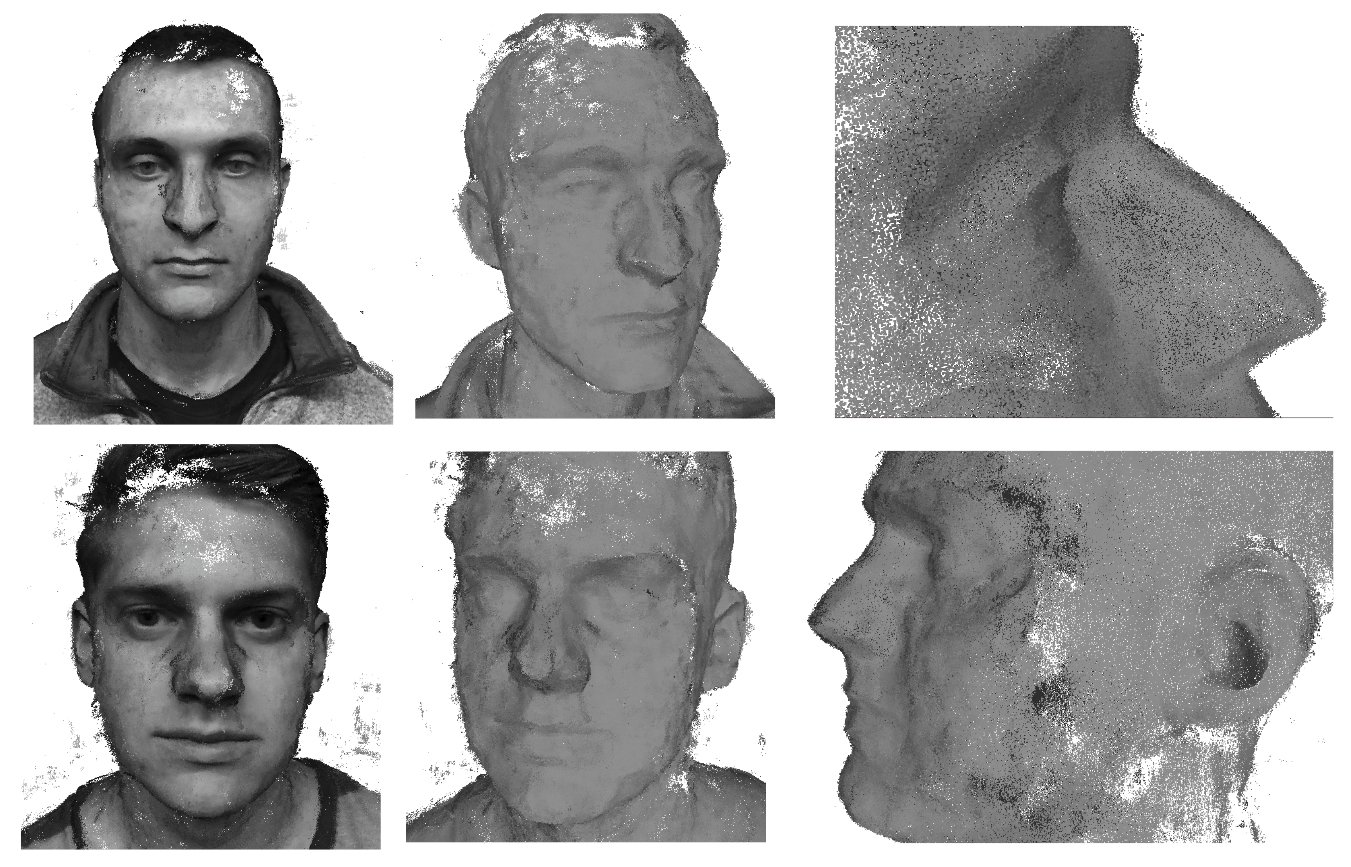
\includegraphics[width=0.95\linewidth]{images/point_clouds_sample.png}
\end{center}
   \caption{Example point clouds generated at the end of our Point cloud generation stage. The point clouds accurately capture the overall face geometery and a lot of details in areas like eyes and lips, that make the person recognizable. However, the point clouds have missing data as well as noise, which requires a robust mesh fitting approach, discussed in section \ref{sec:mesh_fit}  }
\label{fig:pcl_sample}
\end{figure}

%-------------------------------------------------------------------------
\subsection{Mesh fitting} \label{sec:mesh_fit}


Due to factors like non-ideal lighting, lack of texture and sensor noise of the smartphone, the obtained point cloud typically has noise and incompletions, with the points distributed around the `true' surface.
 Techniques like screen poisson reconstruction or the depth map fusion strategy of \cite{hernandez2015near} either return meshes with lots of surface noise, or extremely smoothed out details, depending on the regularization used (see Fig. \ref{fig:mesh_comp}. Further, for the reconstructed mesh to be of use in further downstream tasks such as animation, biometrics or as input to a learning algorithm, it is extremely desirable for the meshes to have a consistent topology. \\
 \begin{figure}[t]
\begin{center}
   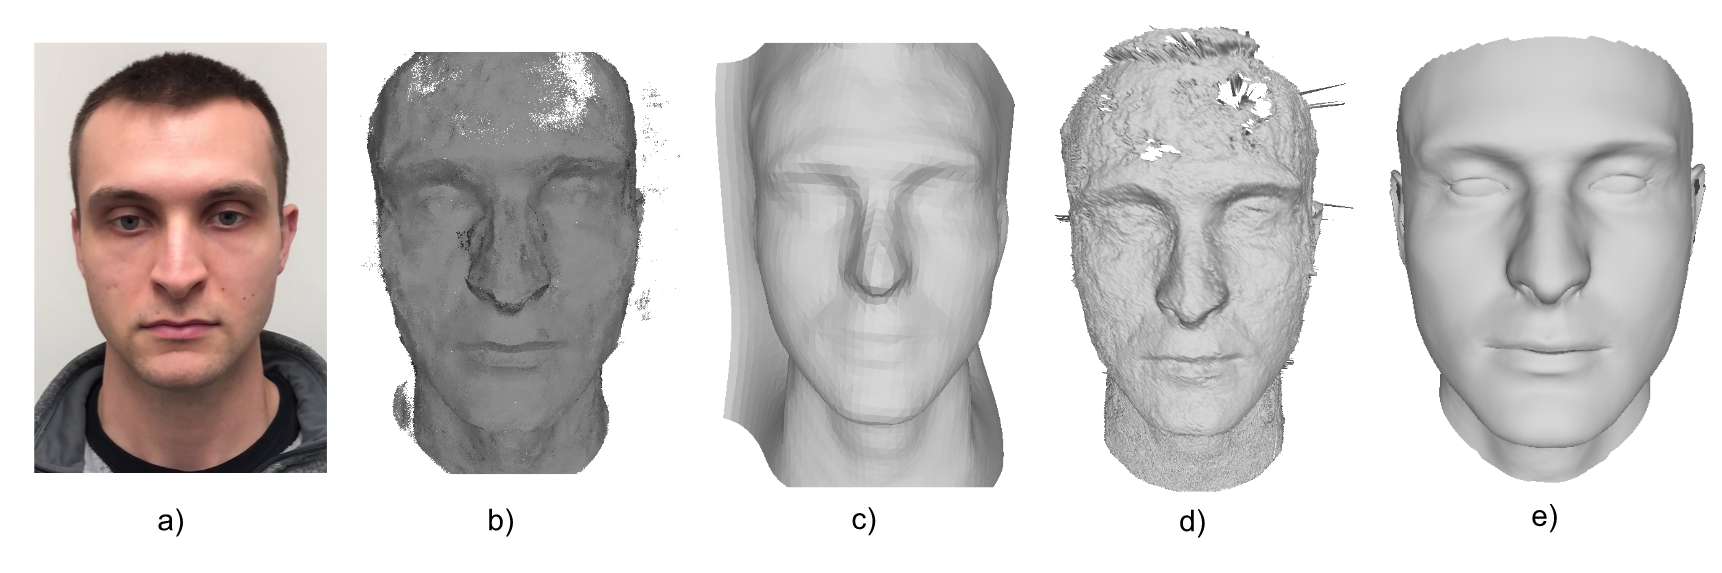
\includegraphics[width=0.95\linewidth]{images/meshing_compare.png}
\end{center}
   \caption{Comparison of mesh generation methods from the reconstructed point cloud. a) Sample image b) generated point cloud c) Screened Poisson Surface Reconstruction\cite{kazhdan2013screened} can fill in gaps in the point cloud but at the cost of overly smooth meshes. d) The depth fusion strategy proposed in \cite{hernandez2015near} can preserve details, but is unable to handle missing data. e) Our approach reconstructs meshes with consistent topology and correspondence between vertices, while capturing details of the point cloud and being robust to noise and missing data }
\label{fig:mesh_comp}
\end{figure}

 Previously, techniques inspired from statistical ICP have proposed fitting. However, this defeats the purpose of not being constrained to an existing linear basis of shape.
 We thus adapt the non-rigid mesh fitting algorithm of \cite{amberg2007optimal}, originally proposed for register template meshes to 3d scanner data, to deform a template using a combination of constraints given by the point cloud, landmarks, mesh stiffness and edge constraints. 
 \subsubsection{Point cloud and landmark constraints}
 The primary constraint for the mesh deformation comes from the 3D information captured in the point cloud and landmarks.
 While well studied techniques exist to register a template mesh to a 3D scanned mesh \cite{amberg2007optimal}, registering a mesh to point clouds of the sort obtained from multi-view stereo techniques is more challenging. 
 
 Thus for each vertex on the template mesh we obtain its desired location in 3D as the median of these points. \\
 
 The other source of information are the 68 2D landmarks obtained using the automatic landmarking solution of \cite{baltrusaitis2018openface}. For the set of frames for which the landmarks have been annotated with high confidence by the tracker (typically close to frontal poses), we solve for the 3D locations of the landmarks by minimizing geometric reporjection error, 
 \begin{equation}
    E_{X_{j}} = \sum_{i} \sum_{j} d(\pi (\theta_{i},X_{j}),x_{ij})^2
\end{equation}
Where $\theta_i$ is the $i$-th camera's pose, $X_{j}$ is the $j$-th landmark's coordinates in 3D, and $x_{ij}$ is the 2D coordinate of the landmark returned by the landmark tracker for the $i$-th frame. For our purposes, we ignore the 18 landmarks corresponding to the face contour, and use the remaining 50 landmarks as additional constraint for the corresponding 3D vertices. 


 \begin{figure}[t]
\begin{center}
   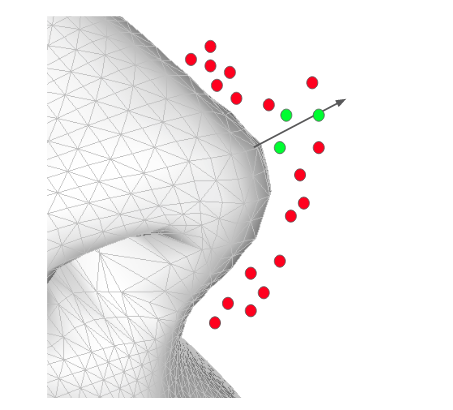
\includegraphics[width=0.8\linewidth]{images/mesh_fit_pcl.png}
\end{center}
   \caption{Exaggerated view of the point cloud fitting. For each vertex, the set of points within a small threshold of its normal (in green here) are found and their median used as the target 3D coordinate for the vertex. }
\label{fig:mesh_fit_pcl}
\end{figure}


\subsubsection{Edge constraints}
Sihouette constraints have shown to be powerful cues in recent 3D reconstruction literature \cite{alldieck2018detailed,bas2016fitting}. For faces, views that are close to profile are particularly informative. However, since many single and multi-view approaches rely on landmarking for camera pose estimation, they fail to make use of silhouettes beyond a certain angle.
However, as noted earlier, by solving for the camera poses independently of landmarking, we can actually make use of extreme profile views, which contain a lot of information for  areas that have typically proven to be challenging for face reconstruction algorithms, such as the nose, lips and lower chin/neck region.
We use a combination of Z-buffering \cite{Foley1990ComputerG} and backface-culling  to estimate vertices that project an edge onto a given view. To find the corresponding edges in the RGB image, we use the Structured Forests edge detection approach proposed in \cite{dollar2013structured}. The corresponding point is backprojected in 3D to obtain a `target' in 3D for the vertex.
T for each vertex corresponding to an 

\subsubsection{Ear Landmarking}

Almost all face reconstruction techniques are reliant on detecting keypoints on the face images, typically using the landmarks for aligning and estimating a course mesh shape.
Historically, most landmark trakers have focused on the ibug 68 landmark scheme \cite{}, since it has the most data available for training learning based models. As a consequence, many reconstruction techniques either only focus on reconstructing the frontal face region, or generate a full mesh but evaluate only on the frontal section. Ears and the side facial regions have historically been completely ignored. Even deep learning based face alignement techniques do not do well on the ears, as the underlying training data is based on the ibug landmarks. This often leads to bad mesh (figure) bad alignment . 
To explicity address this, we make use of a recent dataset by . We then train an ensemble of regression trees \cite{} for predicting landmarks using the bounding box detection as input. Despite the limited training data size, we are able to achieve
To the best of our knowledge, ours is the first face reconstruction method to explicity address the ears, which in turn improves overall accuracy and metrics like the width of the face.

\begin{figure}[t]
\begin{center}
   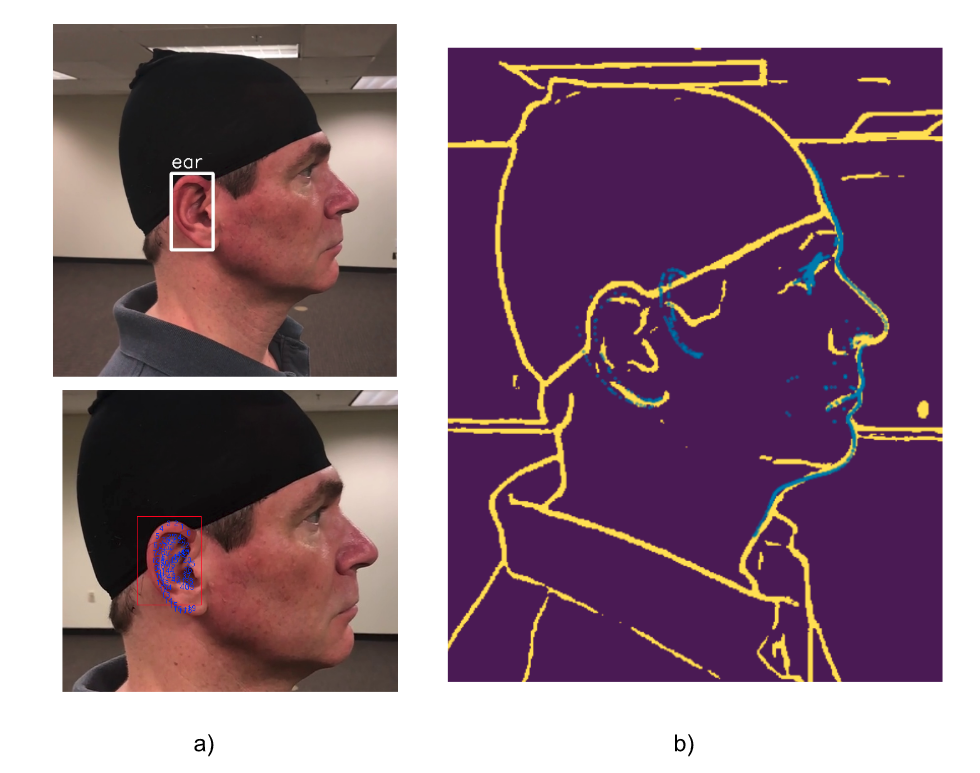
\includegraphics[width=0.95\linewidth]{images/ear_lm_and_edges.png}
\end{center}
   \caption{ a) We train a bounding box and landmark detector specifically for ears. This improves our reconstructions's overall accuracy while allowing us to capture ear size and contour. b) Visualization of edge constraints. Edges in rgb image are shown in yellow, mesh vertices projected in blue. Note that our mesh fits the ears well because of the landmark detection }
\label{fig:ear_lm_and_edges}
\end{figure}


 \subsubsection{Putting it all together}
 
 
 At each iteration, a linear system of the form AX=B is solved, where X is a 4x4n matrix the per vertex 4x4 transform matrix. The matrix A is a stack of  and the source vertices. The matrix B contains the corresponding `target' locations in 3D. The mesh stiffness and the weights of the landmarks is gradually decreased, gradually moving from global stretching to local,data driven deformations. For further details we refer the reader to the orignal paper by Amberg et al. For our template, we use the Basel 3DMM mesh \cite{blanz1999morphable}, simply beacuse of its prevalence as an input or output of several face reconstruction algorithms.

% \begin{table}
% \begin{center}
% \begin{tabular}{|l|c|}
% \hline
% Method & Frobnability \\
% \hline\hline
% Theirs & Frumpy \\
% Yours & Frobbly \\
% Ours & Makes one's heart Frob\\
% \hline
% \end{tabular}
% \end{center}
% \caption{Results.   Ours is better.}
% \end{table}

%---------------------------



\subsection{Mesoscopic Augmentations}

\begin{itemize}
    \item Previous work on "dark-is-deep" assumption. Mention learnt mesoscopic and studio requirement
    \item Mention i2i mesh heat flow for high pass, we propose band pass formulation 
    \item Capture medium scale detail by deforming directly with difference from mean
\end{itemize}
%------------------------------------------------------------------------
%------------------------------------------------------------------------
%-------------------------------------------------------------------------
%------------------------------------------------------------------------

\section{Experiments}

You must include your signed IEEE copyright release form when you submit
your finished paper. We MUST have this form before your paper can be
published in the proceedings.


%%%%%%%%%%%%%%%%%%%%%%%%%%%%%%%%%%%%%%%%%%%%%%%%%%%%%%%%%%%%%%%%%%%%%%%%%%%%%%55
%%%%%%%%%%%%%%%%%%%%%%%%%%%%%%%%%%%%%%%%%%%%%%%%%%%%%%%%%%%%%%%%%%%%%%%%%%%%%%%%5
\subsection{Quantitative Evaluation}

\begin{table*}[t]
\centering
\caption{Quantitative results against ground truth scans. We evaluate the state of the art single and multi-view reconstruction methods. As is common in MVS benchmarks, we evaluate the reconstructions in terms of avarage distance from reconstruction to ground truth (accuracy) and distance from ground truth to reconstruction (completion).}
% \resizebox{\textwidth}{!}{%
\begin{tabular}{c |c| c | c c c}
\hline
Method & Single/Multi-view & Calibration Req. & Accuracy & Completion & Consistency \\
\hline\hline
Furu \cite{furukawa2010accurate}       & 0.612          & 0.939          & 0.775          & 69.37          & 57.97      \\ 
Tola \cite{Tola2011EfficientLM}      & 0.343          & 1.190          & 0.766          & 88.96          & 53.88            \\ 
\hline
SurfaceNet\cite{ji2017surfacenet} & 0.450          & 1.043           & 0.746          & 75.73 & 66.3  \\ 
MVSNet\cite{mvsnet}     & 0.444         & 0.741 & 0.592 & 82.93          & 62.71 \\

\hline
Ours w/o Edges    &  1.565          & 1.378 & 1.472 & 46.90          & 42.16  \\
Ours w/o ear lms    &  1.069          & 1.020 & 1.045 & 55.98          & 45.24\\
Ours    &  0.881          & 1.073 & 0.977 & 61.54          & 44.98 \\


% \specialrule{.16em}{.08em}{.081em}
\hline
\end{tabular}%
% }
\label{table:results}
\end{table*}


\begin{figure*}
\begin{center}
   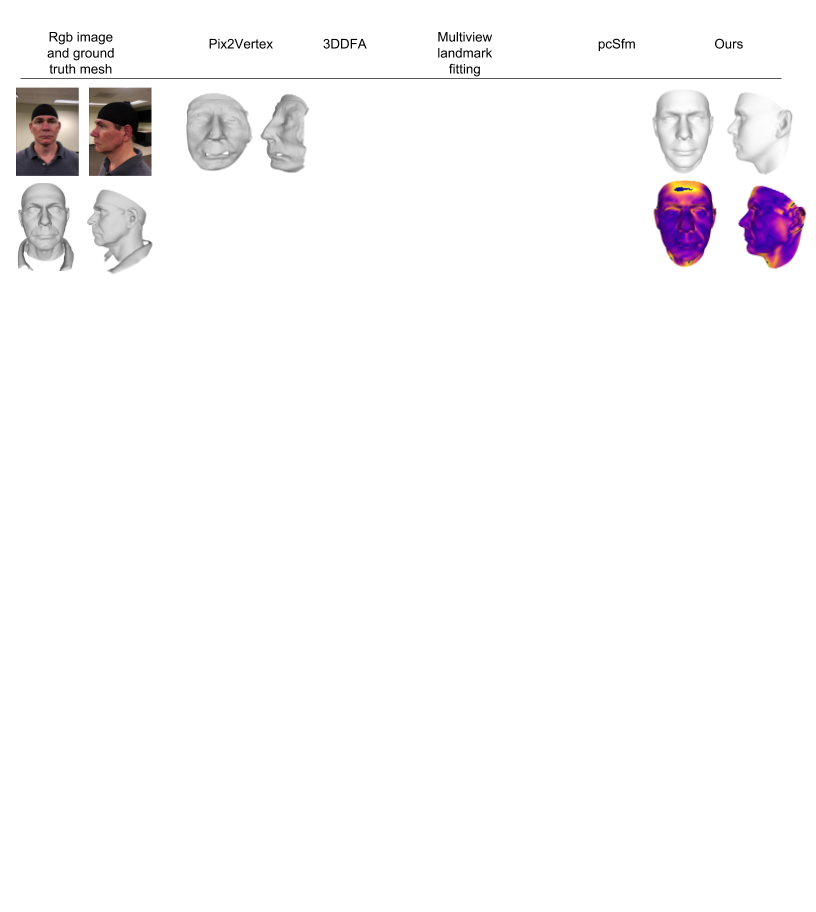
\includegraphics[width=0.95\linewidth]{images/ICCV_verticals.png}
\end{center}
  \caption{Reconstruction and error heat map visualization of various approaches}
\label{fig:results}
\end{figure*}

%%%%%%%%%%%%%%%%%%%%%%%%%%%%%%%%%%%%%%%%%%%%%%%%%%%%%%%%%%%%%%%%%%%%%%%%%%%%%%%%%%%%%5
%%%%%%%%%%%%%%%%%%%%%%%%%%%%%%%%%%%%%%%%%%%%%%%%%%%%%%%%%%%%%%%%%%%%%%%%%%%%%%%%%%%5%%

Maybe mention methods whose number are avaiable but code isnt.

compared to such such and , they only report ( ) and we are better. 
ear     
\subsubsection{Ablation studies}

\subsection{Qualitative evaluation}
\begin{figure}[t]
\begin{center}
% \fbox{\rule{0pt}{2in} \rule{0.9\linewidth}{0pt}}
   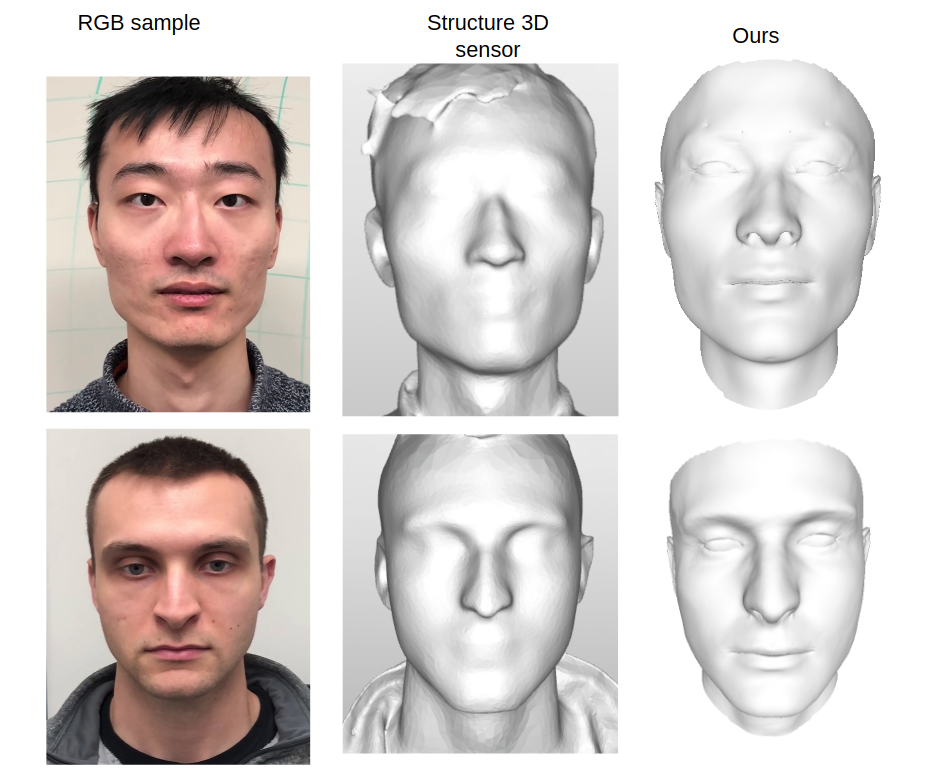
\includegraphics[width=0.9\linewidth]{images/struc_3d_comp.png}
\end{center}
   \caption{Our method reconstructs meshes with more detail than a Structure Sensor, a commercially available low cost IR-based RGB-D scanner \cite{structure2019} specialized for scanning humans. As can be seen, details like the eyes, nose and lips are excessively smoothed out.}
\label{fig:long}
\label{fig:onecol}
\end{figure}

Compare against scan obtained by structure 3d sensor -> comment on better than low cost depth sensor, while being eeve easier for the end user.

\subsubsection{Expressions}

 \begin{figure}[t]
\begin{center}
   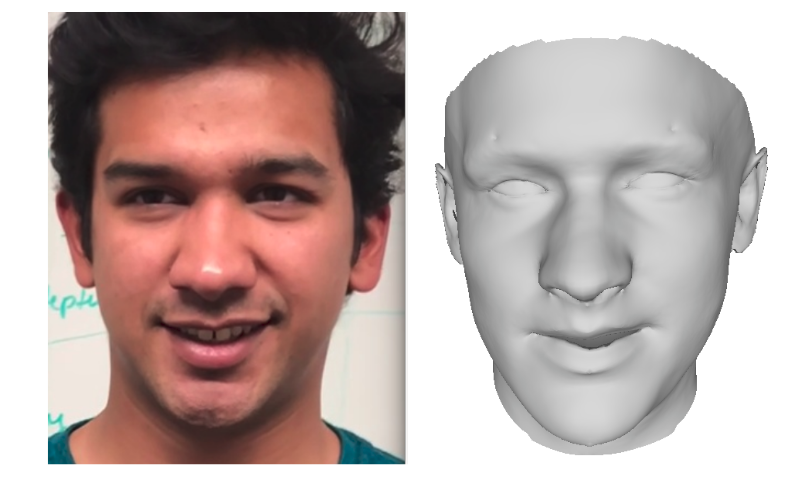
\includegraphics[width=0.8\linewidth]{images/expression_dummy.png}
\end{center}
   \caption{ TEMP, DONT PUT SELF FACE- COLLECT other scans from lab, potentially push to suplementary }
\label{fig:expressions}
\end{figure}

Since our method captures the geometry of the face in a completely data-driven manner, it also generalizes to deformations caused by expressions. 
Since it is difficult to hold the same expression through a video sequence and also obtain a corresponding ground truth 3D, we skip quantitative evaluation of this and provide some qualitative visualizations in Fig \ref{fig:expressions}. 
We also note that since there is dense correspondence and consistent topology across meshes, various existing techniques \cite{} multiv cosistent anchor frames, rigging, animation, blendshapes/warehouse, can be applied with our reconstructed meshes to generate animated, expressive face models.




%%%%%%%%%%%%%%%%%%%%%%%%%%%%%%%%%%%%%%%%%%%%%%%%%%%%%%%%%%%%%%%%%%%%%%%%%%%%%%%%%%%%%%5
%%%%%%%%%%%%%%%%%%%%%%%%%%%%%%%%%%%%%%%%%%%%%%%%%%%%%%%%%%%%%%%%%%%%%%%%%%%%%%%%%
%%%%%%%%%%%%%%%%%%%%%%%%%%%%%%%%%%%%%%%%%%%%%%%%%%%%%%%%%%%%%%%%%%%%%%%
\section{Dataset}
\begin{table}
\begin{center}
\begin{tabular}{|l|c| c|}
\hline
Dataset & \# Subjects & \# Poses \\
\hline\hline
ND-2006 & 888 & None \\
BU-3DFE & 100 & 2 \\
Texas 3DFRD & 118 & None\\
Bosphorus & 105 & 13\\
CASIA-3D & 123 & 11\\
MICC & 53 & Multi*\\
UHDB11 & 23 & 12\\
\hline
\end{tabular}
\end{center}
\caption{An overview of available 3D face datasets and the pose variation in RGB images available in them. Note that although MICC contains videos of subjects with varying pose, the subjects do not hold the same expression through the video, so ground truth for most views is not available}
\end{table}


\begin{itemize}
    \item Maybe add table of existing datasets, resolution, 3d available
    \item  Limited 3d gt data, our experiments reveal severe flaw of deep learning methods trained on synthetic data (pix2vertex), showing very poor generalization to true "in-the-wild" images, with different lighting/noise models then what was use to generate the synthetic data. 
    \item Validated on subset for which ground truth obtained using high accuracy structured light. Rest of the scans are validated using "self-consistency" : for the two sequences of a subject collected under different conditions, the resulting meshes are ensured to be similar up to a tolerance.
    \item Help more interesting deep learning : cite mvsnet / dtu dataset
    \item We provide video, reconstrcuted mesh and 50-100 "keyframes" with known camera poses with respect to the mesh, We also provide the depth map and surface normal map obtaine dusing the mesh
    \item We hope "In the wild" , unconstrained , help train and evaluate robust yet accurate and consistent multi and single view reconstruction algorithms

    \item repeat synthetic data problem, refer to results/images
    \item Self validate others, different lighting conditions

\end{itemize}

\section{Conclusion}
Limitations, importance to community

\newpage
{\small
\bibliographystyle{ieee}
\bibliography{egbib}
}




\end{document}
